% Chapter Template

\chapter{Ensayos y resultados} % Main chapter title

\label{Chapter4} % Change X to a consecutive number; for referencing this chapter elsewhere, use \ref{ChapterX}

En este capítulo se presentan las pruebas realizadas para validar el correcto funcionamiento del sistema implementado. Se incluyen pruebas funcionales de cada bloque en particular y de todo el sistema integrado.

%----------------------------------------------------------------------------------------
%	SECTION 1
%----------------------------------------------------------------------------------------

\section{Pruebas funcionales de hardware}
\label{sec:pruebasHW}

Lastimosamente por los retrasos en el inicio  del proyecto, y los problemas con el envío de las placas electrónicas desde China a Argentina debido a la pandemia de COVID-19, no se pudieron realizar ensayos en el hardware final. Sin embargo, se realizó una prueba con la placa de desarrollo en la que se basó el diseño del proyecto. La misma se muestra en la figura \ref{fig:KDRaytac}.

\begin{figure}[htpb]
	\centering
	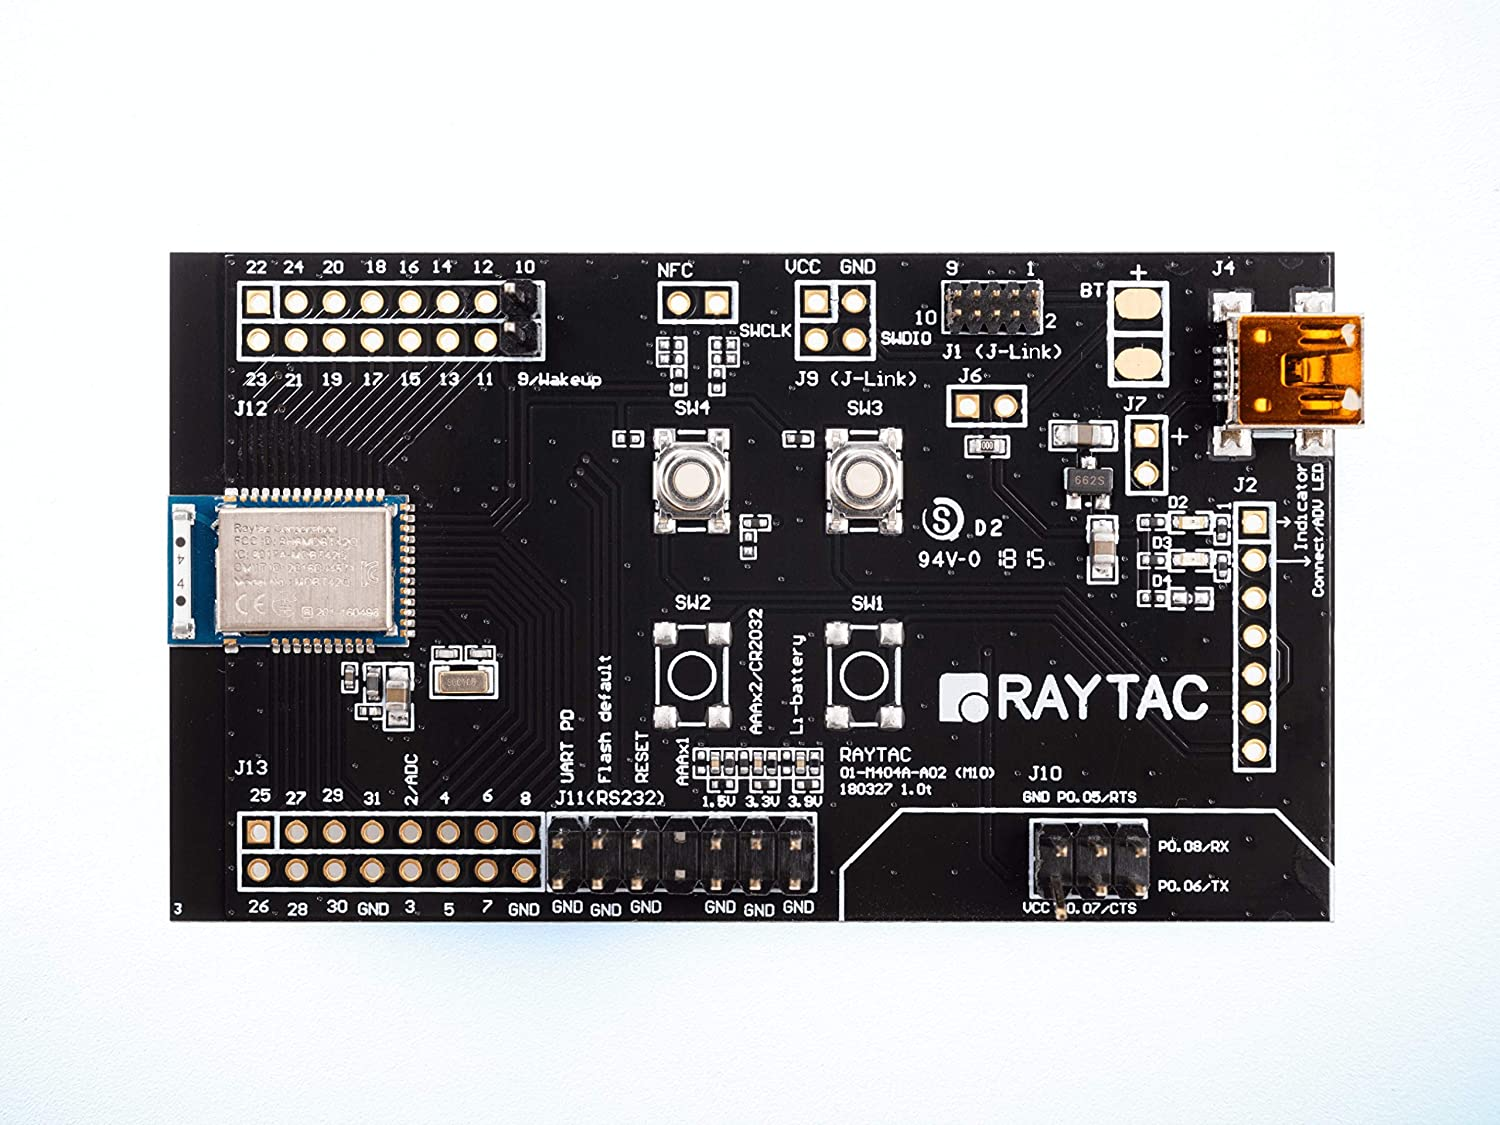
\includegraphics[scale=0.15]{./Figures/DKMDBT42Q-512KV2.jpg}
	\caption{Kit de desarrollo Raytac MDBT42Q-512KV2}
	\label{fig:KDRaytac}
\end{figure}

La prueba se realizó para que SURIX pueda decidir cómo sería la fabricación final de la placa de la central receptora, ya que esta debe estar alojada en los gabinetes en los que la empresa entrega sus productos actualmente, algunos de los cuales tienen una tapa frontal metálica. Esta prueba estaba dirigida a determinar, si el producto final del trabajo, podría ser utilizado en dichos gabinetes sin tener grandes pérdidas de potencia en la señal recibida, En ella, se realizaron mediciones de potencia de señal, tanto con el dispositivo Bluetooth dentro del gabinete metálico, como por fuera de él, para determinar las diferencias.

El gabinete utilizado para esta prueba se puede apreciar en la figura \ref{fig:GMetalico}.

\begin{figure}[htpb]
	\centering
	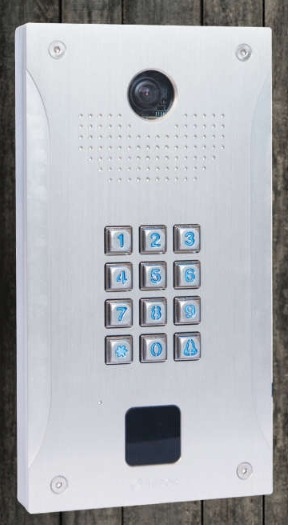
\includegraphics[scale=0.4]{./Figures/gabMet.jpeg}
	\caption{Gabinete metálico SURIX}
	\label{fig:GMetalico}
\end{figure}

Para medir la potencia de la señal se utilizó la aplicación móvil que proporciona Nordic semiconductor, nRFConnect, la cual permite escanear todos los dispositivos Bluetooth que se encuentran dentro del rango de detección del teléfono móvil y muestra la potencia de la señal que recibe de cada uno de ellos.

Los resultados obtenidos se muestran en la figura \ref{fig:Psenal}.

\begin{figure}[!h]
	\centering
   	\begin{subfigure}[b]{0.45\textwidth}
   		\centering
      	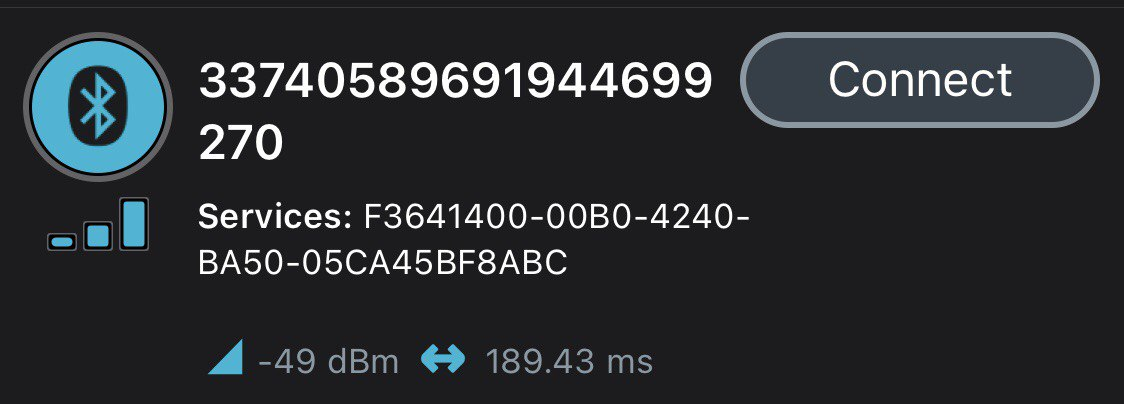
\includegraphics[width=1\textwidth]{signalCO.jpeg}
      	\caption{Medicion a 10 cm de distancia fuera del gabinete}
      	\label{fig:PsenalA}
   	\end{subfigure}%
   	\hfill
   	\begin{subfigure}[b]{0.45\textwidth}
   		\centering
      	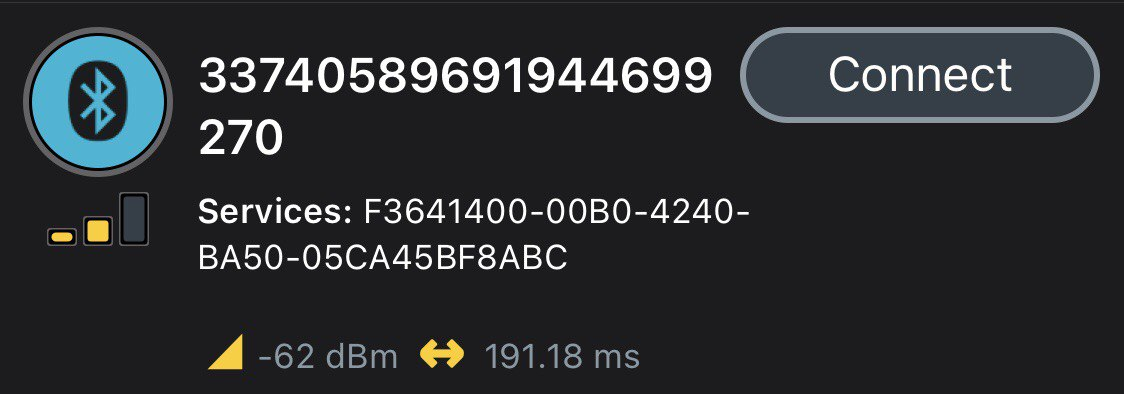
\includegraphics[width=1.03\textwidth]{signalCI.jpeg}
      	\caption{Medicion a 10 cm de distancia dentro del gabinete}
      	\label{fig:PsenalB}
   	\end{subfigure}%
   	\newline
   	\begin{subfigure}[b]{0.45\textwidth}
   		\centering
      	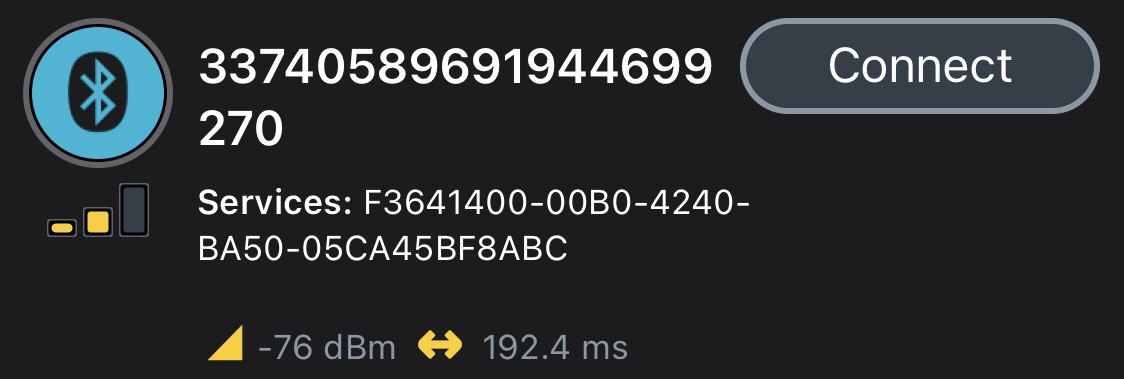
\includegraphics[width=1.04\textwidth]{signalAO.jpeg}
      	\caption{Medicion a 10 m de distancia fuera del gabinete}
      	\label{fig:PsenalC}
   	\end{subfigure}%
   	\hfill
   	\begin{subfigure}[b]{0.45\textwidth}
   		\centering
      	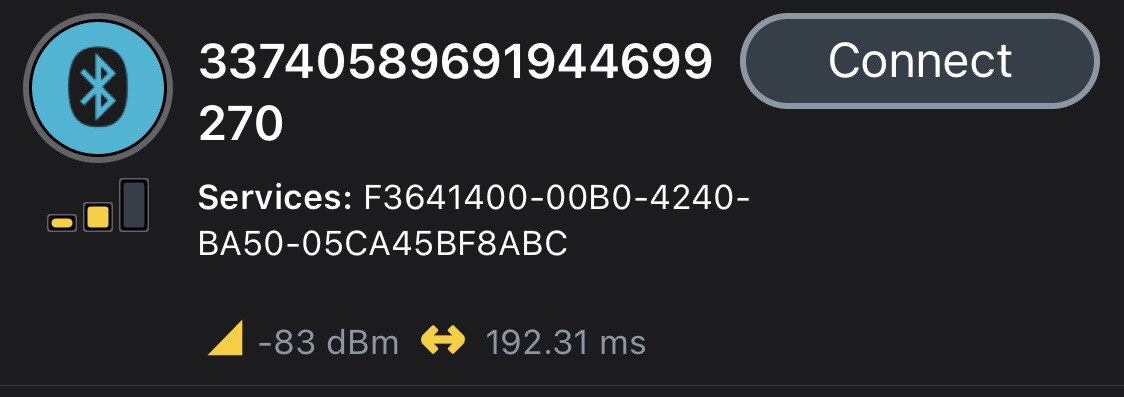
\includegraphics[width=1\textwidth]{signalAI.jpeg}
      	\caption{Medicion a 10 m de distancia dentro del gabinete}
      	\label{fig:PsenalD}
   	\end{subfigure}%
	\caption{Resultados medición potencia de señal recibida del módulo de Bluetooth}
	\label{fig:Psenal}
\end{figure}

En los apartados \ref{fig:PsenalA} y \ref{fig:PsenalB} de la figura se observan las mediciones a 10 cm de distancia del dispositivo Bluetooth dentro y fuera del gabinete metálico respectivamente, existiendo una pérdida de 13 dBm. Y en los apartados \ref{fig:PsenalC} y \ref{fig:PsenalD} se ven las mediciones realizadas a 10 metros de distancia del dispositivo, donde se aprecia una pérdida de tan sólo 7 dBm, por lo que se concluye que las pérdidas son pequeñas y no afectarán a la comunicación.

Finalmente, para determinar de forma práctica que el dispositivo se podría utilizar con estos gabinetes metálicos, se hizo un último ensayo estableciendo una llamada tal como ocurriría  en condiciones reales de uso al interior de una sala de hospital.

Para esto se instaló una placa Bluetooth dentro del gabinete de la figura \ref{fig:GMetalico}, y se la conecto al terminal de sala, que a su vez se conectó a una red local para poder establecer una llamada con un ordenador, en el cual se dispone de softphone (software que permite establecer llamadas VoIP en un ordenador). Por otro lado se usó otro dispositivo Bluetooth con el micrófono conectado y se estableció una llamada con el ordenador.

Los resultados de este ensayo fueron positivos, ya que no se presentaron dificultades durante la llamada, y se escuchó claramente la voz recibida por Bluetooth.

\section{Pruebas unitarias}
\label{sec:pruebasUN}

Las pruebas unitarias se realizaron para cada módulo, conforme se fueron desarrollando, empezando por los más básicos y aquellos que servirían de base para otros.
Para la comunicación Bluetooth, en todos los servicios implementados para el funcionamiento del sistema, cada servicio se implementó y probó, siempre primero del lado del dispositivo llamador, ya que este cumple el rol de periférico, para luego implementar y probar del lado de la central receptora.

Para validar los resultados obtenidos en la central receptora, se hizo uso de la UART del dispositivo, y se reenvió todo lo que se recibía de los servicios por esta interfaz. Para comprobar la correcta recepción de los datos, se conectó el módulo de Bluetooth con el que se realizaron las pruebas, a un adaptador de TTL a USB que permite ver los resultados en el ordenador usando el software cutecom, que no es más que un terminal serial para la PC.

El primer servicio que se probó fue el servicio UART de Nordic, que si bien es un servicio incluido en el paquete de desarrollo de Nordic se decidió hacer la prueba para comprobar que la implementación fue correcta en el firmware. 

Los resultados del lado del llamador se probaron haciendo uso de las aplicaciones de Nordic para móvil: nRFconnect y nRF Toolbox, con la primera se verificó que el servicio ya estaba presente, y con la segunda que al presionar un botón el dispositivo llamador efectivamente enviaba el mensaje programado. Los resultados de esta prueba se muestran en la figura \ref{fig:Pnus}.

\begin{figure}[htpb]
	\centering
   	\begin{subfigure}[b]{0.5\textwidth}
   		\centering
      	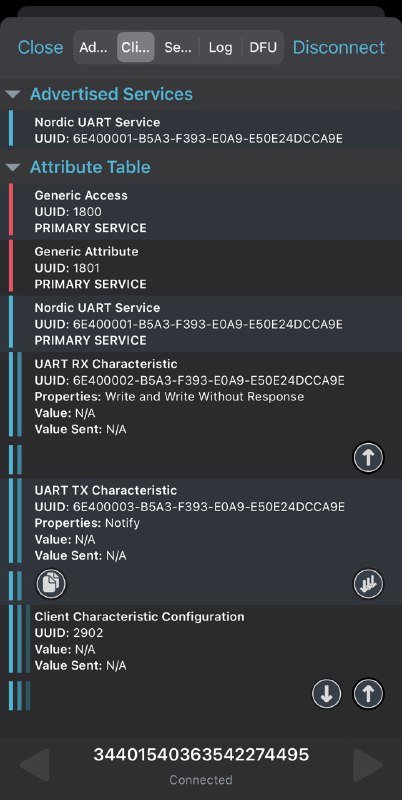
\includegraphics[width=0.8\textwidth]{nusCC.jpeg}
      	\caption{Servicio reconocido en nRFConnect}
      	\label{fig:PnusA}
   	\end{subfigure}%
   	\begin{subfigure}[b]{0.5\textwidth}
   		\centering
      	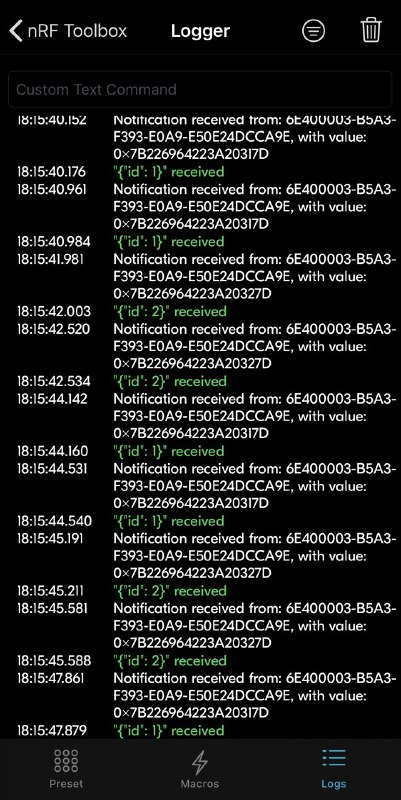
\includegraphics[width=0.8\textwidth]{nusCT.jpeg}
      	\caption{Mensajes recibidos en nRF Toolbox}
      	\label{fig:PnusB}
   	\end{subfigure}%
	\caption{Resultados prueba servicio NUS en el dispositivo llamador}
	\label{fig:Pnus}
\end{figure}

Una vez probado el servicio UART de Nordic en el dispositivo llamador, se probó que también funcionara en la central receptora. Se probó con dos llamadores conectados, para verificar que podía aceptar la conexión de varios periféricos, y que recibía los mensajes de este servicio. Los resultados de esta prueba se muestran en la figura \ref{fig:Pnus2}.

\begin{figure}[htpb]
	\centering
	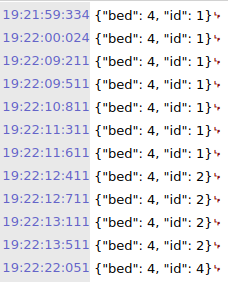
\includegraphics[scale=0.7]{./Figures/Pnus2.png}
	\caption{Resultados prueba servicio de NUS en la central receptora}
	\label{fig:Pnus2}
\end{figure}

El siguiente servicio probado  fue el servicio de audio, pero estas pruebas se exponen en el apartado \ref{sec:pruebasACS} debido a que se implementó desde cero y es el servicio más importante del sistema.

Posteriormente se probó el servicio de batería, que es el encargado de notificar el nivel de carga de batería del dispositivo llamador. Este servicio, al igual que el NUS, viene ya implementado en el paquete de desarrollo de Nordic.

Para probarlo se hizo uso de las dos aplicaciones móviles antes mencionadas, otra vez verificando que el servicio sea reconocido, y que el valor de carga de la batería pueda ser leído. Los resultados de esta prueba se muestran en la figura \ref{fig:Pbas}.

\begin{figure}[htpb]
	\centering
   	\begin{subfigure}[b]{1\textwidth}
   		\centering
      	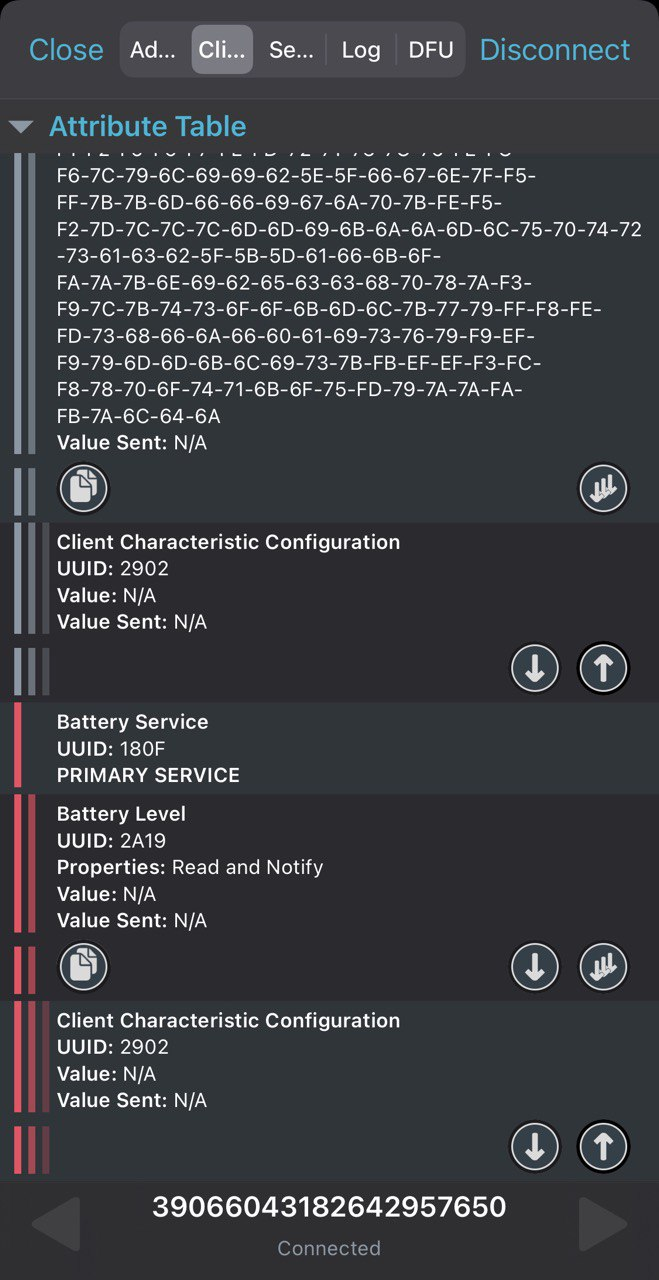
\includegraphics[width=0.5\textwidth]{basCC.jpeg}
      	\caption{Servicio reconocido en nRFConnect}
      	\label{fig:PbasA}
   	\end{subfigure}%
   	\newline
   	\begin{subfigure}[b]{1\textwidth}
   		\centering
      	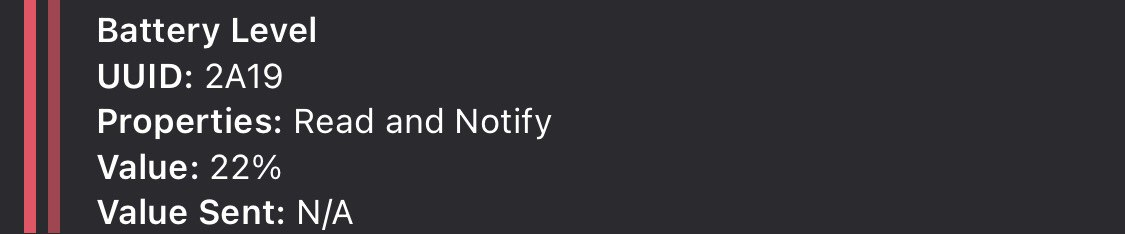
\includegraphics[width=0.7\textwidth]{basCT.jpeg}
      	\caption{Mensajes recibidos en nRF Toolbox}
      	\label{fig:PbasB}
   	\end{subfigure}%
	\caption{Resultados servicio de batería en el dispositivo llamador}
	\label{fig:Pbas}
\end{figure}

Para terminar con la parte bluetooth se probó el servicio de batería en la central receptora, verificando que recibía los niveles de batería y que los notificara por UART si el nivel de batería estaba por debajo del 25\%. Los resultados de esta prueba se muestran en la figura \ref{fig:Pbas2}, y se pueden verificar la notificación con un mensaje con id 3.

\begin{figure}[htpb]
	\centering
	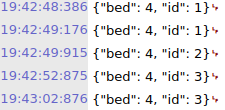
\includegraphics[scale=0.7]{./Figures/Pbas2.png}	
	\caption{Resultados servicio de batería en la central receptora}
	\label{fig:Pbas2}
\end{figure}

Con los servicios de bluetooth probados, se procedió a implementar y probar el módulo de control de la placa expansora. Lo primero que se probó fue que en la web se incluyan los campos para registrar los identificadores de los dispositivos llamadores, y que teniendo registrado algún valor se manden los identificadores por la UART del terminal. Los resultados se muestran en la figura \ref{fig:Pllam}.

\begin{figure}[htpb]
	\centering
   	\begin{subfigure}[b]{1\textwidth}
   		\centering
      	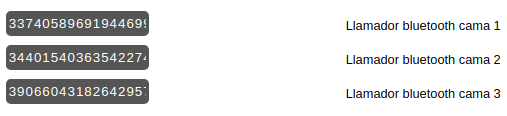
\includegraphics[width=0.8\textwidth]{regcall.png}
      	\caption{Llamadores registrados en pagina web de la terminal de sala}
      	\label{fig:PllamA}
   	\end{subfigure}%
   	\newline
   	\begin{subfigure}[b]{1\textwidth}
   		\centering
      	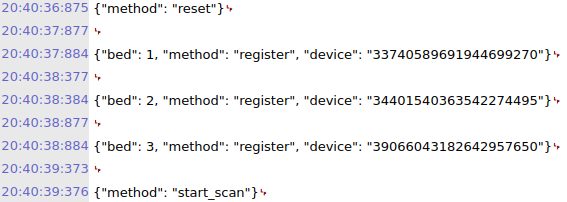
\includegraphics[width=0.8\textwidth]{regcall1.png}
      	\caption{Mensajes enviados para registrar llamadores en central receptora}
      	\label{fig:PllamB}
   	\end{subfigure}%
	\caption{Resultados del registro de identificadores de los dispositivos llamadores}
	\label{fig:Pllam}
\end{figure}

\section{Pruebas de envío y recepción de audio por Bluetooth}
\label{sec:pruebasACS}

Para el envío y recepción de audio, no se tenía ningún servicio disponible en el paquete de desarrollo de Nordic, razón por la cual se implementó desde cero y se realizaron pruebas según se fue implementando. 

Para empezar se desarrolló un driver para controlar el micrófono con la interfaz PDM. Para verificar el funcionamiento de esta interfaz, se utilizó un analizador lógico que permitió ver las señales de reloj y de datos que se recibían del micrófono. Los resultados obtenidos se muestran en la figura \ref{fig:Ppdm}.

\begin{figure}[htpb]
	\centering
	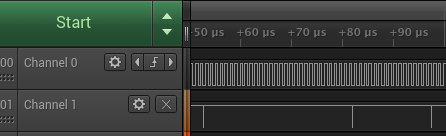
\includegraphics[scale=0.8]{./Figures/pdm.png}	
	\caption{Resultados driver de microfono PDM}
	\label{fig:Ppdm}
\end{figure}

Con la interfaz funcionando, la siguiente tarea fue probar que el servicio implementado en el dispositivo llamador fuera reconocido en la aplicación nRFconnect. Una vez verificado que  el servicio era reconocido, se comprobó que al activar la notificación del servicio los datos del micrófono se puedan ver en la misma aplicación. Los resultados se muestran en la figura \ref{fig:Pacs}.

\begin{figure}[htpb]
	\centering
	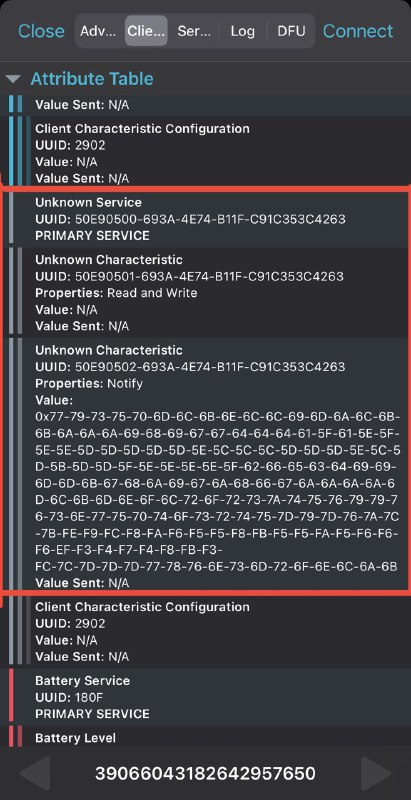
\includegraphics[scale=0.5]{./Figures/acsCC.jpeg}	
	\caption{Resultados servicio de audio en el dispositivo llamador}
	\label{fig:Pacs}
\end{figure}

Del lado de la central receptora se probó que los datos se reciben en el nuevo servicio, y que se pasan directamente a través de UART. La primera prueba de este servicio, fue que los datos del micrófono se pudieran ver en el software cutecom mencionado en el apartado 4.2. Los resultados se muestran en la figura \ref{fig:Pacs2}.

\begin{figure}[htpb]
	\centering
	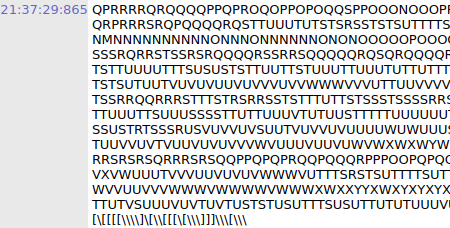
\includegraphics[scale=0.5]{./Figures/acsCR.png}	
	\caption{Resultados servicio de audio en central receptora}
	\label{fig:Pacs2}
\end{figure}

La segunda prueba realizada con los datos recibidos por UART, fue graficar en tiempo real los datos del micrófono, para ello se desarrolló un software en Python. Esta prueba se realizó para comprobar que la onda generada por los datos recibidos, cambiaba en función a los estímulos que recibía el micrófono. Los resultados fueron positivos y se muestran en la figura \ref{fig:Psau}.

\begin{figure}[htpb]
	\centering
	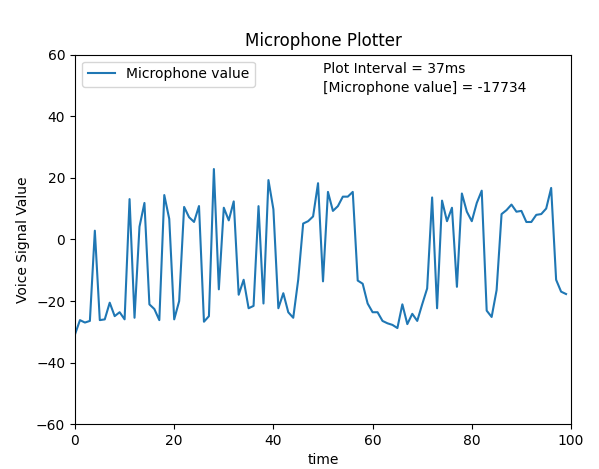
\includegraphics[scale=0.6]{./Figures/callpython.png}	
	\caption{Grafica señal de audio recibida del dispositivo llamador}
	\label{fig:Psau}
\end{figure}

Finalmente, se hizo que los datos del micrófono se envíen al terminal de sala y, que éste los envíe directamente al parlante que tiene conectado. Los resultados finales fueron satisfactorios.

\section{Pruebas de integración}
\label{sec:pruebasInt}

La última etapa de prueba del proyecto fue probar el funcionamiento de todo el sistema en su conjunto. Para verificar esto se registraron dos identificadores correspondientes a dos dispositivos llamadores, que para las pruebas fueron los módulos de desarrollo con los que se trabajó el proyecto.

Para comprobar que los dispositivos llamadores fueron correctamente registrados, después de tener inicializada la central receptora, se comprobó que los llamadores efectivamente se conectaron a la misma, verificando que estuviera encendido el LED indicador de conexión. A continuación, en la figura \ref{fig:Pmcon} se evidencia el estado de conexión de los dispositivos llamadores.

\begin{figure}[htpb]
	\centering
	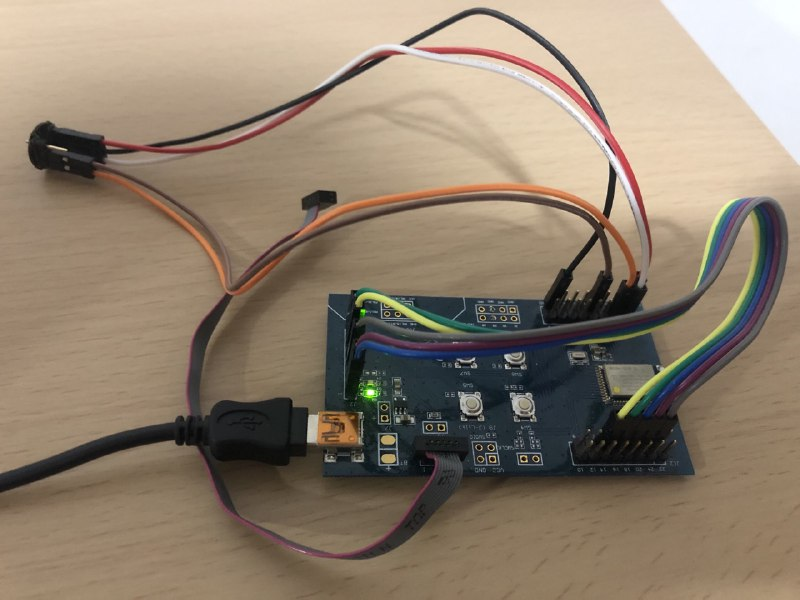
\includegraphics[scale=0.45]{./Figures/callcon.jpeg}	
	\caption{Dispositivo llamador conectado}
	\label{fig:Pmcon}
\end{figure}

Posteriormente, con un analizador lógico conectado en paralelo a la interfaz UART del terminal de sala, se probó que al presionar un botón de uno de los dispositivos llamadores la central receptora reaccionara notificando del evento indicando el número de cama al que está registrado el llamador que originó la novedad. En la figura \ref{fig:Pmrcv} se muestra el resultado de esta prueba.

\begin{figure}[htpb]
	\centering
   	\begin{subfigure}[b]{1\textwidth}
   		\centering
      	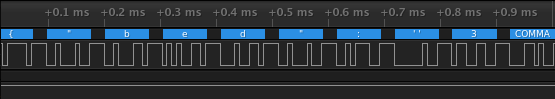
\includegraphics[width=1\textwidth]{intRcv.png}
      	\caption{Mensaje recibido en el terminal de sala}
      	\label{fig:PmrcvA}
   	\end{subfigure}%
   	\newline
   	\begin{subfigure}[b]{1\textwidth}
   		\centering
      	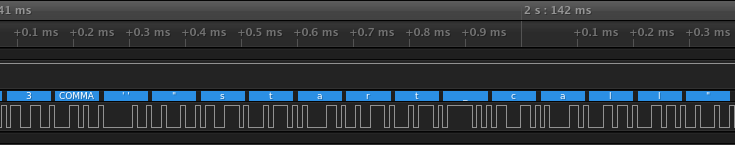
\includegraphics[width=1\textwidth]{intSend.png}
      	\caption{mensaje envido por el terminal de sala al dispositivo llamador}
      	\label{fig:PmrcvB}
   	\end{subfigure}%
   	\newline
   	\begin{subfigure}[b]{1\textwidth}
   		\centering
      	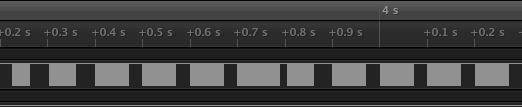
\includegraphics[width=1\textwidth]{intAu.png}
      	\caption{Señal de audio recibida por el terminal de sala}
      	\label{fig:PmrcvC}
   	\end{subfigure}%
	\caption{Mensajes recibidos por el terminal de sala}
	\label{fig:Pmrcv}
\end{figure}

Finalmente la última prueba realizada al sistema fue iniciar una llamada con uno de los llamadores. En la figura \ref{fig:Pmicon} se evidencia un segundo led encendido indicando que el llamador tiene encendido su micrófono, y en la figura \ref{fig:Psrtp} se observa la imagen de una captura de paquetes de la señal de audio que viaja por RTP durante la llamada.

\begin{figure}[htpb]
	\centering
	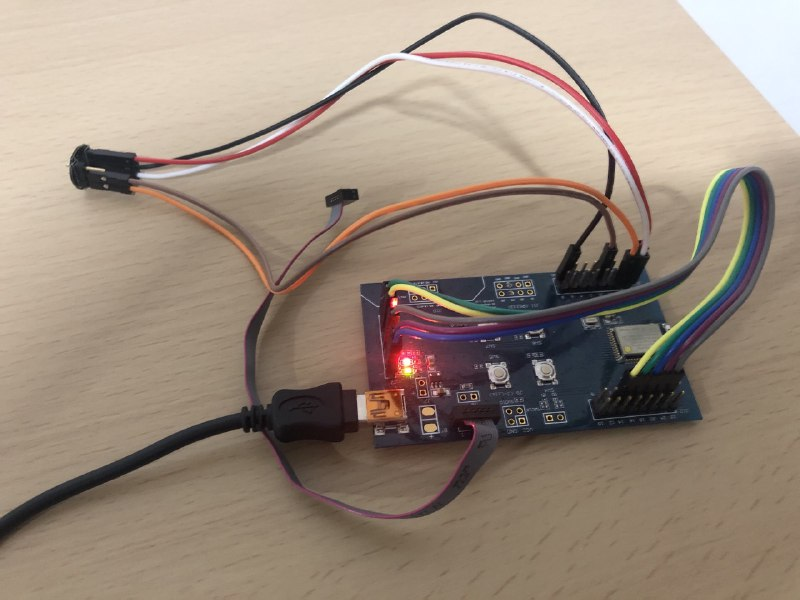
\includegraphics[scale=0.45]{./Figures/callCtrue.jpeg}	
	\caption{Llamador durante llamada en curso}
	\label{fig:Pmicon}
\end{figure}

\begin{figure}[htpb]
	\centering
   	\begin{subfigure}[b]{1\textwidth}
   		\centering
      	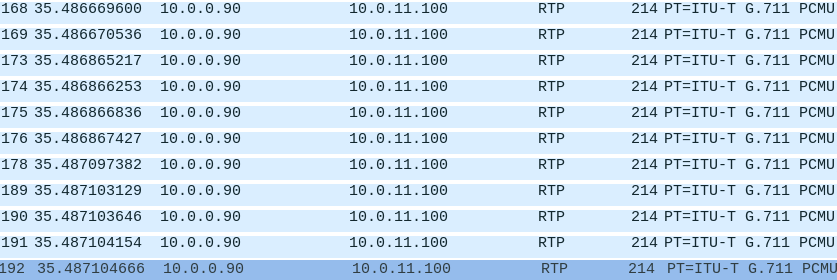
\includegraphics[width=1\textwidth]{rtp.png}
      	\caption{Paquetes RTP enviados por el terminal de sala}
      	\label{fig:PsrtpA}
   	\end{subfigure}%
   	\newline
   	\begin{subfigure}[b]{1\textwidth}
   		\centering
      	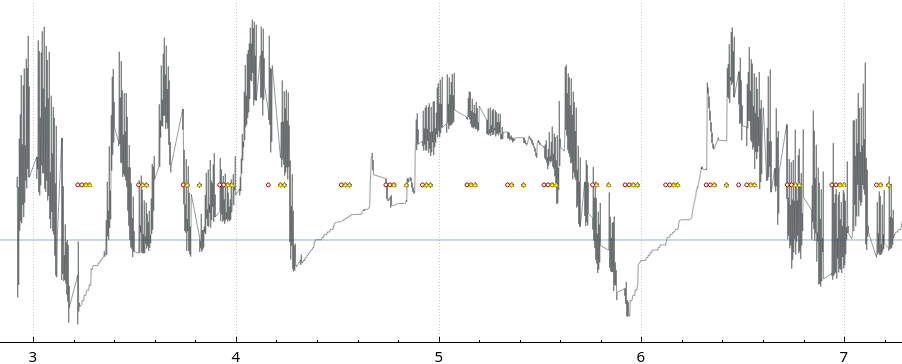
\includegraphics[width=1\textwidth]{rtpStream.png}
      	\caption{Grafica paquetes RTP enviados por el terminal de sala}
      	\label{fig:PsrtpB}
   	\end{subfigure}%
	\caption{Señal de voz enviada durante llamada}
	\label{fig:Psrtp}
\end{figure}

\section{Resultados del trabajo}
\label{sec:resTrab}

En coordinación con SURIX se realizó una demostración del funcionamiento del sistema a los ejecutivos, al personal de las áreas de ingeniería y producción de la empresa. Como conclusión de dicha demostración podemos afirmar que los resultados obtenidos fueron satisfactorios, ya que tanto los ejecutivos como el personal de la empresa manifestaron su satisfacción y beneplácito con el producto.

En otro contexto, para evidenciar las mejoras del sistema respecto al anterior, en la tabla \ref{tab:sistemasDeLLamadoEnfermera2} se compara las características de este nuevo sistema de la empresa SURIX con los productos existentes en el mercado, mencionados en el apartado \ref{sec:AntyCont}. 

\begin{table}[h]
	\centering
	\caption[Sistemas de llamado a enfermera]{Tabla comparativa de los sistemas de llamado a enfermera disponibles en el mercado}
	\begin{tabular}{l c c c c}    
		\toprule
		\textbf{Característica} 	 & \textbf{SURIX} & \textbf{MMCALL} & \textbf{Helpnex} & \textbf{SEI}\\
		\midrule
		Dispositivo llamador inalámbrico                                                    & X &   &   & X \\
Central de enfermera inalámbrica                                                    & X & X & X & X \\
\begin{tabular}[c]{@{}l@{}}Aviso de presencia de \\ enfermera por RFID\end{tabular} & X &   & X &   \\
Sistema de localización de pacientes                                                &   &   & X &   \\
Panel de control                                                                    & X & X & X & X \\
Alarma de pasillo configurable                                                      & X & X & X &   \\
Emisión de informes                                                                 & X & X & X &   \\
		\bottomrule
		\hline
	\end{tabular}
	\label{tab:sistemasDeLLamadoEnfermera2}
\end{table}
